\documentclass[A4paper, 12pt]{article}
\usepackage{fancyhdr}
\usepackage{graphicx}
\usepackage{booktabs}
\usepackage{pdfpages}
\usepackage[utf8]{inputenc}
\usepackage[greek,english]{babel}
\usepackage{alphabeta}
\pagestyle{fancy}
\lhead{Vulcano 2.0: μια νέα αρχή}
\rhead{v2.03}
\cfoot{\thepage}
\renewcommand{\headrulewidth}{0.4pt}
\renewcommand{\footrulewidth}{0.4pt}
\addto\captionsenglish{% Replace "english" with the language you use
  \renewcommand{\contentsname}%
    {πίνακας περιεχομένων}%
}
\begin{document}
\title{Vulcano 2.0: μια νέα αρχή}
\author{The Vulcano Team}
\date{\today}
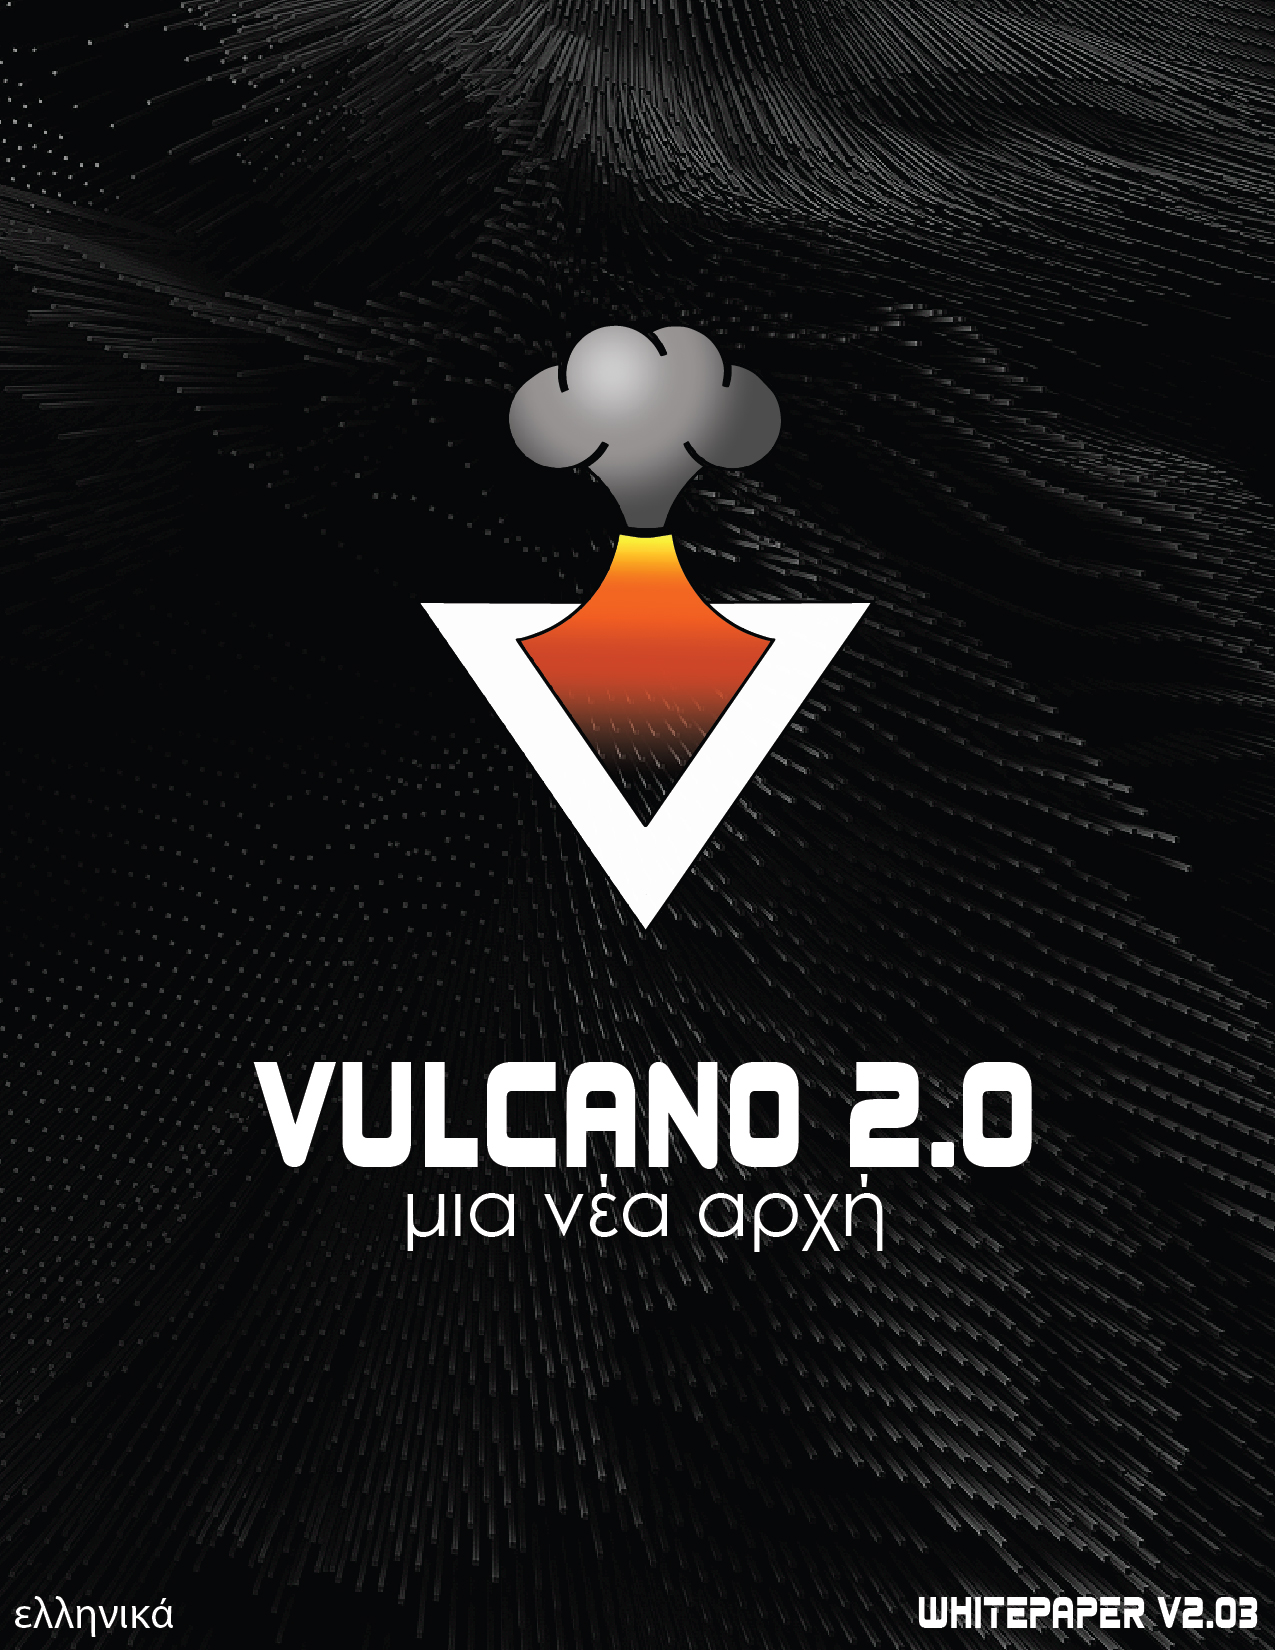
\includepdf[pages=1]{COVER-GRE.jpg}
\newpage
\tableofcontents
\newpage
\section{Εισαγωγή}

Το Vulcano (κωδικός: VULC) είναι ένα νόμισμα κοινοτικού χαρακτήρα που δημιουργήθηκε πρώτη φορά στα τέλη του 2017 από μια ομάδα προγραμματιστών, η οποία είναι παντελώς απούσα πλέον. Η αρχική ιδέα αφορούσε ένα νόμισμα "υψηλής συμμετοχής" με ετήσια απόδοση 950\%. Ωστόσο, λόγω αρκετών λαθών από μέρους της αρχικής ομάδας ανάπτυξης του Vulcano, η πραγματική απόδοση ήταν πιο κοντά στο 320,000\%. Το γεγονός αυτό πέρασε απαρατήρητο, μέχρι τη στιγμή που ένα μέλος της κοινότητας υπολόγισε αυτό το ενεργό πραγματικό επιτόκιο εξετάζοντας την αλυσίδα μπλοκ (blockchain) από το πρώτο μπλοκ συναλλαγών (genesis block). Από τη στιγμή που αποκαλύφθηκε αυτή η θεμελιώδης αδυναμία, η νέα ομάδα του Vulcano - αποτελούμενη από μέλη της κοινότητας - ένωσε τις δυνάμεις της για να διασώσει αφενός το πρότζεκτ Vulcano τόσο σε τεχνικό όσο και σε φιλοσοφικό επίπεδο, μέσα από μια διαδικασία πλήρους αναδόμησης, αφετέρου προχωρώντας στην ανάπτυξη μιας πραγματικής περίπτωσης χρήσης. Σε αυτό το έγγραφο περιγράφεται η στρατηγική για τη συνολική αναβάθμιση του Vulcano και την επανακυκλοφορία του νέου, αναβαθμισμένου νομίσματος ως μέσου χρηματοδότησης γεωθερμικών εξερευνήσεων και ερευνών.

Αντί απλά να διορθώσουμε το πρόβλημα με το επιτόκιο του Vulcano, επιλέξαμε να αναβαθμίσουμε πλήρως το νόμισμα σε μια νέα βάση κώδικα. Προκειμένου να εκσυγχρονίσει με τον καλύτερο δυνατό τρόπο τον πυρήνα του Vulcano, η αρμόδια ομάδα αποφάσισε να χρησιμοποιήσει το Bulwark ως βάση κώδικα. Το Bulwark βασίζεται στο PIVX, το οποίο με τη σειρά του βασίζεται στο δημοφιλές κρυπτονόμισμα DASH. Αυτή η σημαντική απόφαση θα μας δώσει τη δυνατότητα να υλοποιήσουμε κυρίαρχους κόμβους (masternodes) και σχετικές λειτουργίες διαχείρισης, έτσι ώστε στην πορεία η ενσωμάτωση των υλικών κόμβων να μπορεί να υποστηρίζει το οικοσύστημα του Vulcano. Με αυτόν τον τρόπο, θα δημιουργήσουμε ένα πραγματικά αποκεντρωμένο σύστημα διαχείρισης, εξασφαλίζοντας παράλληλα υψηλό επίπεδο ασφάλειας σε ό,τι αφορά τη συμμετοχή στο νόμισμα (stake) και τη δικτυακή σύνδεση.

Η παρούσα εργασία παραθέτει, επίσης, τα μελλοντικά σχέδια για την εδραίωση του Vulcano μέσα από την ίδρυση του Vulcano Foundation, μιας μη κερδοσκοπικής οντότητας κατά το άρθρο 501(c)3, με έδρα στις Η.Π.Α., η οποία θα δώσει στο Vulcano τη δυνατότητα να αναπτυχθεί και να ωριμάσει, ώστε να αρχίσει να συνδέεται και να διαπραγματεύεται με τον υπόλοιπο επιχειρηματικό κόσμο. Αυτό είναι ιδιαίτερα σημαντικό, καθώς η μακροπρόθεσμη περίπτωση χρήσης του Vulcano απαιτεί την απόκτηση ενός χαρτοφυλακίου πνευματικών δικαιωμάτων μέσω της χρηματοδότησης πανεπιστημιακών ερευνών και ερευνητικών ινστιτούτων σε όλο τον κόσμο. Το Vulcano Foundation θα μας επιτρέψει να αξιοποιήσουμε με τον καλύτερο δυνατό τρόπο αυτήν την πνευματική ιδιοκτησία. Πρόκειται για ένα εξαιρετικά κρίσιμο βήμα που θα δώσει στο αποκεντρωμένο πρότζεκτ Vulcano τη δυνατότητα να αλληλεπιδρά και να συνδέεται με τους κεντρικοποιημένους κόσμους των επιχειρήσεων και των πανεπιστημίων.

Αυτή η εργασία παραθέτει, επίσης, τα προβλεπόμενα ποσοστά για τις χρεώσεις διαχείρισης, οι οποίες θα χρησιμοποιούνται για τη χρηματοδότηση γεωθερμικών ερευνών με σκοπό την επιστημονική πρόοδο αλλά και την απόκτηση πνευματικών δικαιωμάτων, και κατ' επέκταση την προσέλκυση περισσότερης χρηματοδότησης προς το Vulcano Foundation για τη μελλοντική του ανάπτυξη και την παροχή κεφαλαίων για επιπρόσθετες επιχορηγήσεις.

Αυτό που δεν θα βρείτε σε αυτήν την εργασία είναι ακραίες και αβάσιμες υποσχέσεις για το μέλλον του blockchain του Vulcano. Η ομάδα του Vulcano πασχίζει για την καινοτομία και την ανάπτυξη, χωρίς να δίνει υποσχέσεις που δεν θα μπορεί να τηρήσει. Αντίθετα, θα επικεντρώσουμε όλες μας τις προσπάθειες στην έρευνα και την προώθηση της τεχνολογικής προόδου. Όλη η τεχνολογία για το blockchain που αναφέρεται στην παρούσα εργασία έχει παρουσιαστεί ήδη στο παρελθόν και θα τεθεί σε λειτουργία εν καιρώ. Πιστεύουμε ότι οι κοινότητες των κρυπτονομισμάτων πρέπει να αρχίσουν πλέον να δρουν κατά τέτοιο τρόπο ώστε να συνάδει με την επιχειρηματική τους δυναμική. Δεν χρειάζονται ακραίες δηλώσεις για την τεχνολογία του blockchain, για να δημιουργηθεί ένα επιχειρηματικό πλάνο για τη χρήση της υπάρχουσας τεχνολογίας. Οι προγραμματιστές, οι επικεφαλείς των ομάδων και οι ίδιες οι κοινότητες πρέπει να κατανοήσουν ότι, προκειμένου να γίνουμε αποδεκτοί από τις ευρύτερες επιχειρηματικές και ακαδημαϊκές κοινότητες, θα πρέπει να είμαστε πρόθυμοι να ακολουθήσουμε τους δικούς τους κανόνες, μέχρι ενός σημείου, και να χρησιμοποιήσουμε αποτελεσματικά όσα διαθέτουμε, πριν αρχίσουμε να προωθούμε ιδέες για μη αποδεδειγμένες τεχνολογίες blockchain, οι οποίες δεν έχουν καν αναπτυχθεί, δοκιμαστεί ή σχεδιαστεί. Παρότι μπορεί να υπάρξουν εξελίξεις και στην τεχνολογία του blockchain για το ίδιο το Vulcano στο μέλλον, η κυκλοφορία αυτής της τεχνολογίας δεν θα συνοδευτεί από πολύμηνους εορτασμούς και διαφημιστικές ενέργειες. Θα μιλήσουμε γι' αυτήν μόνο εφόσον θα έχει αναπτυχθεί. Πιστεύουμε ότι αυτή η μέθοδος της "υπόγειας" ανάπτυξης είναι προς όφελος του νομίσματος, καθώς περιορίζει τις κερδοσκοπικές επενδύσεις και επιτρέπει τη δημιουργία σταθερών θεμελίων για το μέλλον της πλατφόρμας.

Ο στόχος μας είναι να μετατρέψουμε το Vulcano σε μία από τις βασικές πηγές χρηματοδότησης των ερευνών για βιώσιμες πηγές ενέργειες στο μέλλον και, κατά συνέπεια, να δημιουργήσουμε ένα επιχειρηματικό οικοσύστημα γύρω από αυτήν την τεχνολογία.

\section{Συντελεστές}
Το Vulcano δεν θα μπορούσε να έχει υλοποιηθεί χωρίς την προϋπάρχουσα εργασία των αντίστοιχων ομάδων των Bitcoin, Peercoin, Blackcoin, Talkcoin, Dash, PIVX και, κυριότερα, του Bulwark. Καθώς η νέα μορφή του Vulcano αποτελεί μια τροποποιημένη έκδοση (fork) του Bulwark, έχουμε δανειστεί αρκετές ενότητες από το αντίστοιχο τεχνικό έγγραφο σχετικά με τις λειτουργίες που θα συμπεριλάβουμε χωρίς να τροποποιήσουμε την υπάρχουσα βάση κώδικα. Η ομάδα του Vulcano θεώρησε ότι ήταν προς όφελος της διαφάνειας να συμπεριλάβει αυτές τις ενότητες ως έχουν στο τεχνικό έγγραφο του Bulwark, αντί να τις ξαναγράψει ισχυριζόμενη ότι αποτελούν αυθεντικό περιεχόμενο. Παρότι είναι σημαντικό να αναπτύσσουμε, ως κοινότητα, σταθερές περιπτώσεις χρήσης και επιχειρηματικές δομές που μπορούν να σταθούν σε ευρύτερο επίπεδο, οφείλουμε να προστατέσουμε και να διατηρήσουμε παράλληλα το ήθος του ανοιχτού κώδικα που βρίσκεται πίσω από τα κρυπτονομίσματα. Η ανταλλαγή πληροφοριών είναι επωφελής για όλη την ανθρωπότητα και είμαστε υπερήφανοι που συμβάλλουμε σε αυτό το αναπτυσσόμενο σώμα γνώσεων. Με αυτό ακριβώς το πνεύμα, θα προσφέρουμε και τις τεχνολογίες που θα αναπτυχθούν με τη χρηματοδότηση του ιδρύματος Vulcano Foundation στα έθνη που συμβάλλουν στο οικοσύστημά μας.

BitBender ευχαριστεί τον @Kris Ninakos για τη σκληρή δουλειά του - είναι πραγματικά φίλος της κοινότητας!

\section{Μια σύντομη εισαγωγή στα κρυπτονομίσματα}
Παρότι οι προτάσεις για την τεχνολογία κατανεμημένου μητρώου (distributed ledger) χρονολογούνται από τα τέλη της δεκαετίας του 1980, το πρώτο πραγματικό blockchain γεννήθηκε με τη δημοσίευση μιας μελέτης σε έναν άγνωστο πίνακα ανακοινώσεων για θέματα κρυπτογραφίας, με τίτλο Bitcoin: A Peer-to-Peer Electronic Cash System, από έναν συγγραφέα με το ψευδώνυμο Satoshi Nakamoto. Το blockchain λειτουργεί προσθέτοντας διαδοχικές χρονικές σημάνσεις (timestamps) στις συναλλαγές και "κλειδώνοντάς" τις σε μπλοκ, τα οποία επικυρώνονται με διάφορες μεθόδους, έτσι ώστε να μην είναι δυνατή η αθέμιτη μεταβολή τους. Το Bitcoin, όπως και πολλά άλλα κρυπτονομίσματα, Λειτουργούν με τον λεγόμενο όρο "απόδειξη εργασίας" (proof of work), το οποίο σημαίνει ότι χρησιμοποιούν την υπολογιστική ισχύ ως πηγή σπανιότητας στο δίκτυό τους.

Ωστόσο, δεδομένου ότι το Vulcano επικεντρώνεται σε θέματα βιωσιμότητας και έρευνας στο ενεργειακό πεδίο, μια τέτοια μη βιώσιμη μέθοδος έρχεται σε αντίθεση με τις προσπάθειές μας για ενίσχυση της βιωσιμότητας. Κατά συνέπεια, επιλέξαμε να λειτουργούμε επί της βάσης "απόδειξης συμμετοχής" (proof of stake), όπου η πηγή της σπανιότητας στο δίκτυο είναι τα ίδια τα token. Επιπλέον, με την κυκλοφορία του αναβαθμισμένου Vulcano 30 ημέρες μετά τη δημοσίευση αυτού του εγγράφου, θα διαθέτουμε επίσης κυρίαρχους κόμβους (masternodes), οι οποίοι αποτελούν μια κάπως πιο προηγμένη έκδοση της μεθόδου απόδειξης συμμετοχής, καθώς υπολογιστές σε όλο τον κόσμο όχι μόνο συντηρούν το δίκτυο, αλλά αναλαμβάνουν και κάποιο απλό υπολογιστικό φορτίο. Αυτή τη στιγμή, αυτό το υπολογιστικό φορτίο είναι ελάχιστα μεγαλύτερο από αυτό που αναλογεί στη λειτουργία ενός απλού πορτοφολιού (wallet), αλλά θα θέλαμε να χρησιμοποιήσουμε αυτό το δίκτυο στο μέλλον για σκοπούς κατανεμημένης υπολογιστικής στη βιομηχανία των ανανεώσιμων πηγών ενέργειας, με σκοπό την επίλυση υπολογιστικών προβλημάτων χημείας και φυσικής. Αυτή είναι μια σημαντική προσθήκη στο μακροπρόθεσμο πλάνο για το Vulcano, καθώς τα τμήματα γεωφυσικής και γεωθερμίας των ερευνητικών πανεπιστημίων δεν έχουν, κατά κανόνα, εξίσου καλή χρηματοδότηση με άλλα, πιο "δημοφιλή" πεδία και επομένως δυσκολεύονται περισσότερο να εξασφαλίσουν τον απαιτούμενο χρόνο χρήσης μεγάλων υπολογιστών για την εκτέλεση των προσομοιώσεών τους.

Επιπλέον, από καταναλωτική άποψη, με μεσοδιάστημα 20 δευτερολέπτων μεταξύ των μπλοκ, την καθολική συναίνεση των masternodes, το "κλείδωμα" των συναλλαγών, ένα ελεγχόμενο και σταθεροποιημένο χρονοδιάγραμμα διάθεσης και φιλική προς το περιβάλλον συμμετοχή, το Vulcano ευελπιστεί να γίνει το πρώτο πραγματικά γρήγορο και λειτουργικό κρυπτονόμισμα που θα έχει απτές επιπτώσεις στον κόσμο μας, αποτελώντας ταυτόχρονα μια καλή επιλογή για τους καταναλωτές αλλά και τους οπαδούς των κρυπτονομισμάτων εν γένει.

\section{Το νέο Vulcano}
\subsection{Αναλυτικές πληροφορίες για το blockchain του νέου Vulcano}

\begin{table}[h]
\centering
\begin{tabular}{@{}ll@{}}
\toprule
Κωδικός & VULC \\ \midrule
Αλγόριθμος & NIST5 \\
Θύρα RPC & 62541 \\
Θύρα P2P & 62543 \\
Μεσοδιάστημα μπλοκ & 90 δευτερόλεπτα \\
Αλγόριθμος δυσκολίας & Dark Gravity Wave v3.0 \\
Μέγεθος μπλοκ & 1MB \\
Εξορυγμένα/Έτοιμα νομίσματα & 67 μπλοκ ($\sim$100 λεπτά) \\
Επιβεβαίωση & 6 μπλοκ ($\sim$9 λεπτά) \\
Κυκλοφορία (1 έτος) & 246,194,250 \\
Κυκλοφορία (5 έτη) & 421,126,225 \\
Περίοδος απόδειξης εργασίας (PoW) & nHeight 60 \\
Περίοδος απόδειξης συμμετοχής (PoS) & nHeight 61 \\
Υποστήριξη πρωτοκόλλων & IPV4, IPV6, TOR \\
PoS & Blackcoin v3.0 PoS \\ \bottomrule
\end{tabular}
\end{table}

\subsection{Διασφάλιση της ενότητάς μας ως κοινότητας}
Το Vulcano ξεκίνησε αρχικά ως κοινοτικό νόμισμα και αυτή είναι μια ιδέα στην οποία πιστεύουμε ολόψυχα. Ακριβώς επειδή είναι κοινοτικό νόμισμα, γνωρίζουμε ότι ο καλύτερος τρόπος για να υποστηρίξουμε την πρόοδο του πρότζεκτ είναι υποστηρίζοντας την κοινότητα στην οποία οφείλουμε την ύπαρξή μας. Θα συνεχίσουμε τις δράσεις, τους διαγωνισμούς και τις άλλες δραστηριότητες που διοργανώνουμε με την κοινότητά μας. Επίσης, θα προάγουμε τη συζήτηση και τη διερεύνηση των ορίων του οικοσυστήματος Vulcano. Σε όλα τα φόρουμ θα ισχύει η πολιτική μας περί μηδενικής ανοχής απέναντι στα περιστατικά παρενόχλησης των νέων μελών, των χρηστών και των άλλων κοινοτήτων κρυπτονομισμάτων. Η ομάδα του Vulcano πιστεύει ότι υπάρχει αρκετός χώρος στον κόσμο των κρυπτονομισμάτων, ώστε να είμαστε σε θέση, αλλά και να επιδιώκουμε, να συνδεόμαστε και να συνεργαζόμαστε αντί να καταστρέφουμε το έργο των άλλων. Παρότι κατανοούμε ότι υπάρχει ένας βαθμός καλοπροαίρετου ανταγωνισμού μεταξύ των οπαδών των διαφόρων πλατφορμών κρυπτονομισμάτων, θα θέλαμε να διασφαλίσουμε ότι όλες οι σχέσεις θα έχουν θετικό χαρακτήρα.

\subsection{Δημιουργία επιχειρηματικών δυνατοτήτων}
Κατά τον χρόνο συγγραφής αυτού του εγγράφου, διαπιστώσαμε ότι ένας μεγάλος αριθμός κρυπτονομισμάτων χρησιμοποιεί παρόμοιο τεχνολογικό υπόβαθρο. Παρότι η υποκείμενη τεχνολογία είναι ακέραια και σταθερή, πολλές φορές ένας βαθύτερος έλεγχος των προδιαγραφών και των παραμέτρων των blockchain αυτών των κρυπτονομισμάτων αποκαλύπτει την υιοθέτηση μάλλον αθέμιτων πρακτικών. Σε άλλες περιπτώσεις, η τεχνολογική υλοποίηση είναι κακή, αλλά η κοινότητα δεν είναι επαρκώς ενημερωμένη ώστε να είναι σε θέση να διαπιστώσει τα προβλήματα, με αποτέλεσμα να μετέχει σε ένα πρότζεκτ που είναι θεμελιωδώς επισφαλές.
Δυστυχώς, το αρχικό Vulcano θα μπορούσε εύκολα να υπαχθεί σε αυτήν την κατηγορία και αυτός είναι ένας από τους βασικούς λόγους που η νέα ομάδα του Vulcano αποφάσισε να αναδιαρθρώσει εκ βάθρων το πρότζεκτ. Πιστεύουμε ότι τα κρυπτονομίσματα θα πρέπει να έχουν πραγματικές επιχειρηματικές εφαρμογές και ότι η τεχνολογία αυτή δεν πρέπει να χρησιμοποιείται αποκλειστικά και μόνο για τη δημιουργία εσόδων από κερδοσκοπικές συναλλαγές για έναν μικρό αριθμό ατόμων που ενεργούν προτού η αγορά κατανοήσει τι πραγματικά συμβαίνει. Πολλές φορές έχουμε δει προγραμματιστές να δημιουργούν ένα κακό νόμισμα, να το προωθούν μέσα από ακριβές διαφημίσεις και έπειτα να το εγκαταλείπουν αφήνοντας "μετέωρη" την κοινότητά τους. Γι' αυτό πιστεύουμε στη διαφάνεια και στην απόδοση ευθυνών. Και γι' αυτό θα διαμορφώσουμε τα απαραίτητα επιχειρηματικά θεμέλια για τη διεξαγωγή πραγματικών επιχειρηματικών συναλλαγών τόσο μέσα στον κόσμο των κρυπτονομισμάτων όσο και έξω από αυτόν.

Κατά συνέπεια, θα ιδρύσουμε αρκετούς επίσημους επιχειρηματικούς οργανισμούς για τη διευκόλυνση αυτών των σχέσεων. Ο πρώτος και σημαντικότερος από αυτούς τους οργανισμούς θα είναι μη κερδοσκοπικός, κατά το άρθρο 501(c)3, και θα ιδρυθεί για τη χρηματοδότηση ερευνητικών πρωτοβουλιών σχετικών με τη γεωθερμία και άλλες συναφείς επιστήμες. Αυτός ο οργανισμός θα είναι υπεύθυνος για την τήρηση όλων των δικαιωμάτων πνευματικής ιδιοκτησίας και των σημάτων επωνυμίας.

Θα δημιουργηθεί, επίσης, μια σειρά εταιρειών περιορισμένης ευθύνης (LLC) για την κάλυψη των τοπικών απαιτήσεων ανά τον κόσμο. Πολλές συναλλαγές με κρυπτονομίσματα απαιτούν την ύπαρξη τοπικής επιχειρηματικής οντότητας και η δημιουργία ενός δικτύου εταιρειών περιορισμένης ευθύνης θα μας παρέχει αυτό ακριβώς. Αυτό το δίκτυο θα δώσει στο ίδρυμα Vulcano Foundation και στην κοινότητα του Vulcano τη δυνατότητα να αναπτύξουν επιχειρηματική δράση σε οποιαδήποτε χώρα του κόσμου, χωρίς να χάσουν την ικανότητά τους να ανταποκρίνονται θετικά στις τοπικές ανάγκες και τις νομικές απαιτήσεις.

\subsection{Υποστήριξη της κοινότητας}
Η κοινότητα VULC είναι ο σημαντικότερος παράγοντας πίσω από τη μακροπρόθεσμη επιτυχία του πρότζεκτ και η ικανότητά της να επηρεάζει ουσιαστικά το μέλλον του νομίσματος και την τεχνολογική ανάπτυξη των βασικών τομέων μας είναι υψίστης σημασίας. Καθώς ο πρωταρχικός μας σκοπός είναι να προάγουμε την έρευνα για τη βιωσιμότητα μέσω της σχεδόν απεριόριστης γεωθερμικής ισχύος που βρίσκεται κάτω από τα πόδια μας, έχουμε θέσει σε εφαρμογή ορισμένα σχέδια για τη χρηματοδότηση των ερευνητών που δραστηριοποιούνται σε αυτούς τους τομείς.

Έτσι, στο τέλος του πρώτου εξαμήνου, στο μπλοκ 172801, σκοπεύουμε να ενεργοποιήσουμε "εκρηκτικά" μπλοκ (Eruption Blocks) στο δίκτυο. Αυτά τα μπλοκ, τα οποία θα πληρώνονται σε μηνιαία βάση, θα δώσουν στην κοινότητα τη δυνατότητα να ασκεί ουσιαστικό έλεγχο επί των ερευνών που χρηματοδοτεί το Vulcano, της ανάπτυξης της επωνυμίας μας και των σχέσεών της. Η καθυστέρηση της ενεργοποίησης αυτού του συστήματος κατά έξι περίπου μήνες θα μας δώσει τον χρόνο να αναπτύξουμε το απαιτούμενο υποκείμενο πλαίσιο για μια θετική εμπειρία χρήσης, επιτρέποντας παράλληλα στο σύστημα να σταθεροποιηθεί μετά τις αλλαγές στον ρυθμό έκδοσης token για μείωση του ποσοστού 320,000\% σε ένα πολύ πιο λογικό ποσοστό.

Επιπλέον, θα επιβληθεί μια χρέωση διαχείρισης 10\% σε όλες τις αμοιβές των μπλοκ, τα έσοδα από την οποία θα χρησιμοποιούνται με διαφανή και ανιχνεύσιμο τρόπο για τη χρηματοδότηση γεωθερμικών ερευνών. Στην πορεία, θα εφαρμόσουμε μια διαδικασία πολλαπλών φάσεων για τη δημιουργία και την υποβολή περαιτέρω προτάσεων, πέραν αυτών που θα επιλέξουμε μόνοι μας. Για να γίνει δεκτή μια πρόταση, θα πρέπει να ολοκληρωθεί πλήρως κάθε βήμα της διαδικασίας επιλογής. Καθώς είναι πεποίθησή μας ότι η σοφία και η γνώση μπορούν να προέλθουν από διάφορες πηγές, προτρέπουμε την κοινότητα του Vulcano να σκεφτεί τις τεχνολογίες που σχετίζονται με τη γεωθερμική ενέργεια. Αφού συγκεντρώσουμε αυτές τις προτάσεις και τις ιδέες, μπορεί να ακολουθήσει ένα στάδιο ψηφοφορίας και συζήτησής τους με τα υπόλοιπα μέλη της κοινότητας, προτού τις εξετάσουμε αναλυτικότερα σε ακαδημαϊκό επίπεδο. Ελπίζουμε ότι η κοινότητα του Vulcano θα είναι σε θέση να προσελκύσει ειδικούς σε θέματα γεωθερμίας από όλο τον κόσμο, οι οποίοι θα συμβάλουν σε αυτή τη διαδικασία.

\subsection{Ρυθμός έκδοσης Vulcano}
Παρακάτω μπορείτε να δείτε τις αμοιβές των μπλοκ και τον ρυθμό έκδοσης (emission rate) για το blockchain του Vulcano.
\begin{table}[h]
\centering
\begin{tabular}{@{}ccccc@{}}
\toprule
Μήνας & Αριθμός μπλοκ & Αμοιβή μπλοκ & Έκδοση & Σύνολο \\ \midrule
0 & 0-1 & 95,000,000 & 95,000,000 & 95,000,000 \\
1-6 & 2 έως 172800 & 500 & 86,396,500 & 181,396,500 \\
7-12 & 172801 έως 345600 & 375 & 64,797,750 & 246,194,250 \\
13-18 & 345601 έως 518400 & 281.25 & 48,598,313 & 294,792,563 \\
19-24 & 518401 έως 691200 & 210.94 & 36,448,734 & 331,241,297 \\
25-30 & 691201 έως 864000 & 158.20 & 27,336,551 & 358,577,848 \\
31-36 & 864001 έως 1036800 & 118.65 & 20,502,413 & 379,080,261 \\
37-42 & 1036801 έως 1209600 & 88.99 & 15,376,810 & 394,457,071 \\
43-48 & 1209601 έως 1382400 & 66.74 & 11,532,607 & 405,989,678 \\
49-54 & 1382401 έως 1555200 & 50.06 & 8,649,456 & 414,639,133 \\
55-60 & 1555201 έως 1728000 & 37.54 & 6,487,092 & 421,126,225 \\
61+ & 1728001 έως το άπειρο & 18.77 & Συνεχίζεται & Συνεχίζεται \\ \bottomrule
\end{tabular}
\end{table}

\subsection{Οι προσπάθειές μας για την καταπολέμηση της κεντρικοποίησης}
Αυτή τη στιγμή, υπάρχουν πολλά ενδημικά προβλήματα στα οικοσυστήματα των blockchain. Τα προβλήματα αυτά, παρότι παρουσιάζονται και σε άλλους τομείς, μπορούν να περιγραφούν σε κάθε περίπτωση ως "υπερβολική κεντρικοποίηση" με τον έναν ή τον άλλον τρόπο.

Το πρώτο είδος κεντρικοποίησης που πρέπει να εξαλειφθεί έχει να κάνει με το γεγονός ότι η συντριπτική πλειοψηφία των διαθέσιμων token ή νομισμάτων βρίσκονται στα χέρια κερδοσκόπων. Αυτό οδηγεί σε εντελώς παράλογες διακυμάνσεις των τιμών, καθώς οι διάφοροι "παίκτες" προσπαθούν να χειραγωγήσουν τις αγορές ενώ οι ελλιπώς ενημερωμένοι κερδοσκόποι αναζητούν την επόμενη ευκαιρία για τη γρήγορη αγορά και πώληση θέσεων. Παρότι η κατάσταση αυτή έχει ελάχιστες, έως και μηδενικές, επιπτώσεις στην πραγματική ανάπτυξη, δημιουργεί την άποψη μέσα στην κοινότητα ότι οι διακυμάνσεις των τιμών προσδιορίζουν ή αντανακλούν, με κάποιον τρόπο, τη θεμελιώδη κατάσταση και πορεία του έργου, ενώ στην πραγματικότητα δεν υπάρχει κανένας απολύτως συσχετισμός μεταξύ τους. Το πρόβλημα της υπερβολικής συγκέντρωσης νομισμάτων από κερδοσκόπους οδηγεί σε αστάθεια και μεγάλα ποσοστά κινδύνου. Ένας από τους στόχους μας είναι να διαχειριστούμε αυτήν την κατάσταση στο μεγαλύτερο δυνατό βαθμό.

Το δεύτερο είδος κεντρικοποίησης έχει γεωγραφικό χαρακτήρα και αφορά τη θέση των εικονικών ιδιωτικών server (VPS) στους οποίους διαμορφώνονται κατά κανόνα οι masternodes. Καθώς υπάρχουν πολλές υπηρεσίες που προσφέρουν φθηνή φιλοξενία masternodes, επικρατεί η τάση να αναπτύσσεται μεγάλος αριθμός κόμβων σε έναν πάροχο. Αυτό σημαίνει ότι ένα και μόνο αναπάντεχο συμβάν μπορεί να καταστρέψει ένα μεγάλο ποσοστό του δικτύου, καθιστώντας το ευάλωτο.

Το ερευνητικό οικοσύστημα του Vulcano προσφέρει μια λύση σε αυτό το "δίδυμο" πρόβλημα της υπερβολικής κεντρικοποίησης. Καθώς το Vulcano Foundation θα χρηματοδοτεί ερευνητικά προγράμματα στον τομέα της γεωθερμίας, αναμένεται σταδιακά να αποκτήσει ένα χαρτοφυλάκιο πνευματικών δικαιωμάτων. Το σχέδιό μας είναι να παρέχουμε αυτήν την πνευματική ιδιοκτησία, έναντι πολύ χαμηλού κόστους, σε κάθε ίδρυμα ή κράτος που θα συμφωνήσει να φιλοξενήσει κόμβους υλικού εξοπλισμού του Vulcano. Με αυτόν τον τρόπο, τα ιδρύματα αυτά θα αποκτήσουν ένα σύνολο τεχνολογικών εργαλείων, τα οποία θα μπορούν να χρησιμοποιήσουν ως βάση για τις δικές τους τεχνολογικές λύσεις, απλά και μόνο καταβάλλοντας το κόστος ανάπτυξης των masternodes στα συστήματά τους ή σε έναν κόμβο υλικού εξοπλισμού του Vulcano. Έτσι, θα μπορέσουμε να διευρύνουμε σημαντικά τη γεωγραφική κατανομή των masternodes του Vulcano, μειώνοντας παράλληλα τα token που είναι ελεύθερα στην κοινότητα και διαθέσιμα για κερδοσκοπικές δραστηριότητες.

Πιστεύουμε, επίσης, ότι είναι σημαντικό να εξασφαλίσουμε την όσο το δυνατόν ευρύτερη διανομή των token του Vulcano. Για την ακρίβεια, πιστεύουμε ότι η πλειοψηφία των μικρότερων πρότζεκτ κρυπτονομισμάτων που έχουν διαθέσει μεγάλα ποσοστά token σε έναν μικρό αριθμό κατόχων αντιμετωπίζουν έναν επικίνδυνο βαθμό κεντρικοποίησης. Κατά συνέπεια, σκοπεύουμε να υλοποιήσουμε ορισμένα σχέδια στο μέλλον, τα οποία θα παρέχουν κίνητρα για την αποκέντρωση και τον κατακερματισμό των μεγάλων wallet, επιβραβεύοντας όσους κατέχουν μικρότερο αριθμό masternodes. Αυτό το θέμα θα συζητηθεί αναλυτικότερα στο μέλλον.

Καθώς η ομάδα του Vulcano υποστηρίζει φανατικά την ανάπτυξη ανοιχτού πηγαίου κώδικα, θα θέλαμε να διατηρήσουμε την ίδια φιλοσοφία σε όσο το δυνατόν περισσότερους τομείς. Φυσικά, το σύνολο των πηγαίου κώδικα θα είναι διαθέσιμο ανά πάσα στιγμή για έλεγχο, αλλά θα θέλαμε επίσης να διαθέσουμε προς χρήση ένα σώμα πνευματικής ιδιοκτησίας με όσο το δυνατόν χαμηλότερο κόστος.

\section{Τα χαρακτηριστικά του Vulcano}
\subsection {Masternodes}
Οι κυρίαρχοι κόμβοι (masternodes), ως σύνολο, αποτελούν ένα αποκεντρωμένο δίκτυο υπολογιστών που υποστηρίζουν τη λειτουργία του δικτύου Vulcano. Οι κόμβοι αυτοί εκτελούν σημαντικές λειτουργίες του δικτύου και λαμβάνουν ένα μέρος των αμοιβών των μπλοκ. Εκτός από την εκτέλεση αυτών των βασικών δικτυακών λειτουργιών, βοηθάνε επίσης σταθεροποιώντας την παροχή νομισμάτων, διεκπεραιώνοντας συναλλαγές και προστατεύοντας το δίκτυο. Η λειτουργία των masternodes απαιτεί 50.000 VULC και μέτρια τεχνική κατάρτιση. Οποιοδήποτε wallet ελέγχει πάνω από 50.000 VULC μπορεί να δημιουργήσει έναν masternode.

Η ομάδα Vulcano έχει μακροπρόθεσμα σχέδια για την εισαγωγή διαφόρων τύπων κόμβων, οι οποίοι θα παρέχουν ανταμοιβές με βάση τη συμβολή τους σε ένα χρήσιμο υπολογιστικό δίκτυο. Με αυτόν τον τρόπο, η δύσκολη διαδικασία της "απόδειξης εργασίας" μπορεί να παραλειφθεί, καθώς οι εκτελούμενοι υπολογισμοί δεν είναι αυθαίρετοι υπολογισμοί που αποσκοπούν στην προστασία του δικτύου και μόνο, αλλά λειτουργικοί υπολογισμοί που συμβάλλουν στην πρόοδο των επιστημών που ασχολούνται με θέματα βιωσιμότητας. Θα δημοσιεύσουμε περισσότερες πληροφορίες σχετικά με αυτήν την πρόταση στο μέλλον, ανάλογα με τις εξελίξεις.

\subsection{Συσκότιση / Συνδυασμός νομισμάτων}
Καθώς ο κώδικας του πυρήνα του νέου Vulcano βασίζεται στο Bulwark, περιλαμβάνει επίσης τη δυνατότητα συσκότισης (obfuscation), η οποία επιτυγχάνεται με αποκεντρωμένο τρόπο και με τη βοήθεια του δικτύου masternodes. Η μέθοδος αυτή παρέχει ένα επιπλέον επίπεδο προστασίας του απορρήτου των συναλλαγών. Παρότι δεν είναι εντελώς ανώνυμη, η συσκότιση μέσω του συνδυασμού κόμβων είναι κατά πολύ ανώτερη των τυπικών συναλλαγών με Bitcoin. Για παράδειγμα, όλες συναλλαγές με Bitcoin είναι διαφανείς και μπορεί κανείς να τις ακολουθήσει εύκολα σε όλο το μήκος του blockchain. Στην περίπτωση του Vulcano, ένας δόλιος "παίκτης" θα έπρεπε να ελέγχει τουλάχιστον το 50\% των λειτουργικών masternodes για να έχει πάνω από 0,5\% πιθανότητες να αποανωνυμοποιήσει μία και μόνο συναλλαγή, η οποία θα έχει περάσει από 8 κύκλους συσκότισης. Αυτή η σημαντική δυνατότητα θα προσφέρει ανωνυμία υψηλού επιπέδου στους χρήστες του VULC που θα επιλέξουν να κάνουν συσκότιση των συναλλαγών τους. Παρότι δεν συνδέεται στενά με την τελική περίπτωση χρήσης του πρότζεκτ Vulcano, προσφέρει έναν βαθμό καταναλωτικής χρησιμότητας που ενισχύει την αξία του σε σχέση με άλλα πρότζεκτ κρυπτονομισμάτων.

\subsection{SwiftTX}
Το SwiftTX προσφέρει στους κατόχους των masternodes την αρμοδιότητα να κλειδώνουν και να επικυρώνουν τις συναλλαγές. Όταν υποβάλλεται μια συναλλαγή στο δίκτυο, η συναλλαγή αυτή επικυρώνεται από μια ομάδα masternodes. Αν επιτευχθεί συμφωνία μεταξύ των masternodes για την εγκυρότητα της συναλλαγής, η συναλλαγή θα κλειδωθεί προκειμένου να εισαχθεί αργότερα στο blockchain, γεγονός που αυξάνει σημαντικά την ταχύτητα των συναλλαγών σε σύγκριση με τα συμβατικά συστήματα (όπως τα μεσοδιαστήματα 10 λεπτών μεταξύ των μπλοκ του Bitcoin με πολλαπλές επιβεβαιώσεις). Το SwiftTX καθιστά εφικτή τη διενέργεια πολλών συναλλαγών πριν την εξόρυξη ενός μπλοκ στο δίκτυο με τα ίδια δεδομένα (input). Το σύστημα αυτό βασίζεται στο InstantSend του Dash.

\subsection{Sporks}
Το δίκτυο του νέου Vulcano χρησιμοποιεί τον μηχανισμό τροποποιήσεων (forking) πολλών φάσεων που χρησιμοποιήθηκε πρώτη φορά στο Bulwark και είναι γνωστός ως "sporking". Ο μηχανισμός αυτός θα βοηθήσει το δίκτυο VULC στην υλοποίηση νέων δυνατοτήτων, ελαχιστοποιώντας παράλληλα τις πιθανότητες ακούσιας τροποποίησης του δικτύου κατά την έναρξη της λειτουργίας του. Οι αλλαγές που γίνονται μέσω spork υλοποιούνται δικτυακά και μπορούν να ενεργοποιηθούν και να απενεργοποιηθούν, ανάλογα με τις ανάγκες, χωρίς να απαιτούνται ενημερώσεις του λογισμικού των κόμβων. Η λειτουργία αυτή είναι εξαιρετικά χρήσιμη και επιτρέπει στο δίκτυο να αντιδρά γρήγορα στις ευπάθειες, χωρίς να απαιτείται η συνδρομή μεμονωμένων χρηστών για τη μη αυτόματη ενημέρωση του κώδικα των wallet τους.

\subsection{TOR \& IPV6 Masternodes}
Το Vulcano θα επιτρέπει στους χρήστες να εκτελούν τα masternodes είτε μέσω μιας διεύθυνσης onion είτε μέσω μιας διεύθυνσης IPV6. Έχουμε ξεκινήσει ήδη τη διαδικασία για την προσθήκη κόμβων TOR με σκοπό την ενίσχυση του ίδιου του δικτύου TOR αλλά και τη βελτίωση της εμπειρίας χρήσης του Bulwark, όταν αυτό χρησιμοποιείται μόνο σε TOR. Ένα μοναδικό πλεονέκτημα που προσφέρει η υποστήριξη masternodes TOR είναι η δυνατότητα λειτουργίας των masternodes ως κρυφής υπηρεσίας TOR. Οι κόμβοι TOR επιτρέπουν στους χρήστες που έχουν σταθερή σύνδεση στο internet να λειτουργούν masternodes από το οικιακό δίκτυό τους, χωρίς να υπάρχει κίνδυνος να αποκαλυφθεί η τοποθεσία τους και χωρίς να εκθέτουν το δίκτυό τους στον κίνδυνο επίθεσης ή παραβίασης.
 
\section{Το μέλλον}
\subsection{Ασφαλής κόμβος υλικού εξοπλισμού Vulcano}
Ορισμένα βασικά στελέχη της ομάδας Vulcano συνεργάζονται ήδη με έναν εξειδικευμένο κατασκευαστή προηγμένου ηλεκτρονικού εξοπλισμού οικιακής χρήσης για την ανάπτυξη κόμβων υλικού εξοπλισμού που θα μπορούν να αναπτυχθούν σε παγκόσμιο επίπεδο, έτσι ώστε να διασφαλίζεται η αποκέντρωση του δικτύου και να παρέχεται μεγαλύτερη ασφάλεια. Οι χρήστες θα μπορούν να συνδέσουν αυτούς τους κόμβους στο οικιακό τους δίκτυο και να τους διαμορφώνουν μέσω ενός διαδικτυακού περιβάλλοντος χρήσης. Ο στόχος μας είναι να παρέχουμε στους χρήστες με σταθερή σύνδεση internet, εύχρηστα και πλήρως αλληλοεπικαλυπτόμενα (onionized) masternodes που θα κάνουν χρήση κρυφών υπηρεσιών TOR.

Ακολουθώντας και εδώ το πνεύμα της αποκέντρωσης, το σύνολο του πηγαίου κώδικα θα είναι διαθέσιμο στα μέλη της κοινότητας, προκειμένου να κάνουν τις απαιτούμενες εργασίες, αλλά παράλληλα θα διατίθεται και ένα έτοιμο μοντέλο. Οι κόμβοι θα είναι επίσης αυτοί που θα διανεμηθούν από το Vulcano Foundation, στο πλαίσιο της προσπάθειάς μας να αυξήσουμε τη γεωγραφική κατανομή και να ενισχύσουμε την ασφάλεια του νομίσματος μέσα από την ανάπτυξη στατικών κόμβων.

\subsection{	Το κατάστημα Vulcano}
Το πρώτο μέλημά μας είναι η δημιουργία μιας ρεαλιστικής περίπτωσης χρήσης για το Vulcano. Ένα πρώτο τέτοιο παράδειγμα θα είναι μια αγορά ψηφιακών αγαθών που θα βασίζεται στο blockchain του Vulcano. Και παρότι στην αρχή τα διαθέσιμα ψηφιακά αγαθά θα προέρχονται από άλλες πηγές, εκτός της κοινότητας, όπως π.χ. κωδικοί και δωροκάρτες Steam, ο στόχος μας είναι να αναπτύξουμε στην πορεία μια peer-to-peer αγορά που θα βασίζεται στο Vulcano.

\subsection{Telegram \& Discord Bots}
Η ψυχή κάθε blockchain είναι η κοινότητα και ένας από τους καλύτερους τρόπους με τους οποίους μπορεί κανείς να υποστηρίξει την κοινότητά του είναι προσφέροντάς της έναν τρόπο επικοινωνίας και χρήσης των token. Η ομάδα του Vulcano θα χρηματοδοτήσει τη δημιουργία bot για διάφορες υπηρεσίες συνομιλίας (chat), έτσι ώστε τα μέλη της κοινότητάς μας να είναι σε θέση να μοιράζονται τα VULC τους εύκολα με τον υπόλοιπο κόσμο. Διευκολύνοντας αυτήν την ελεύθερη ροή του Vulcano, ενισχύουμε τη χρηστικότητά του και παράλληλα συμβάλλουμε στη δραστηριοποίηση και την ανάπτυξη της κοινότητας.

\section{Συμπέρασμα}
Το Vulcano έχει διανύσει ήδη πολύ δρόμο από την ανακάλυψη των κρίσιμων αδυναμιών του πριν από μερικούς μήνες. Η νέα αλυσίδα του Vulcano βρίσκεται ήδη σε στάδιο δοκιμών, έχοντας διευρυμένα χαρακτηριστικά, ενώ έχουν καταβληθεί ήδη σημαντικές προσπάθειες για την αποκατάσταση των προβλημάτων που οδήγησαν στην αποτυχία του αρχικού πρότζεκτ και την αποδυνάμωση της κοινότητας για μήνες. Είμαστε ενθουσιασμένοι που μπορούμε να σας ανακοινώσουμε αυτές τις αλλαγές και να μοιραστούμε μαζί σας τα μακροπρόθεσμα σχέδιά μας. Ανυπομονούμε να μοιραστούμε μαζί σας και νεότερες πληροφορίες, ενημερώνοντας αντίστοιχα το παρόν έγγραφο.

\newpage
\section{Τροποποιήσεις}

\begin{table}[h]
\centering
\begin{tabular}{@{}ccccc@{}}
\toprule
Αριθμός έκδοσης & Ημερομηνία υποβολής & Επεξήγηση \\ \midrule
v2.03 & 8th Αυγούστου 2018 & Πρώτη ελληνική μετάφραση \\
 \bottomrule
\end{tabular}
\end{table}

\end{document}
